%%%%%%%%%%%%%%%%%%%%%%%%%%%%%%%%%%%%%%%%%%%%%%%%%%%%%%%%%%%%%%%%%%
\section{Consistency with partitioned coupling}\label{sec:consistency_partitioned}
%%%%%%%%%%%%%%%%%%%%%%%%%%%%%%%%%%%%%%%%%%%%%%%%%%%%%%%%%%%%%%%%%%
% Stream feeding this section: R2 (campaign/HANDOFF.md), plus the
% womersleyTube runs of R1. Source of the discretisation comparison: audit
% A2, paper-data/a2_discretisation_differences.md (origin/evidence/
% a2-fluid-discretisation-differences), whose draft text is adapted below.

The quasi-monolithic and partitioned couplings in solids4foam solve the same continuum problem with different fluid solvers (\texttt{newtonIcoFluid} and \texttt{pimpleFluid}) and different solid formulations (velocity and displacement), so their solutions should differ only by discretisation error and should approach each other under refinement.
This section states where the two discretisations differ and tests the expectation on a steady and a transient case.
It is a consistency check between two formulations that share much of their code, not an independent verification.

%%--------------------------------------------------------------------------------------------------------------------%%
\subsection{Differences between the discretisations}\label{sec:fluid_differences}
%%--------------------------------------------------------------------------------------------------------------------%%
% Adapted from the draft text at the end of A2. Changes: (i) the traction
% difference (A2 item D6) is presented as an inconsistency that has been
% corrected (solids4foam branch fix/monolithic-deforming-wall-traction,
% Philip's decision of 20 Oct 2026); (ii) recorded pre-tag numbers replaced by
% \tbd placeholders (A2 quotes 0.14/0.08/0.05% for the cavity from
% verification/cavityflexiblebottom-partitioned-fine @ f356c3242).

The two couplings share the solid discretisation, the face interpolation of the stresses and the solid stabilisation, and, for the linear solid, their time integration: the BDF2 velocity formulation with BDF2 kinematics is algebraically identical to the backward second time derivative used by the displacement solid.
They differ in the fluid and at the interface (Table~\ref{tab:discretisation_differences}).
In the fluid, \texttt{newtonIcoFluid} solves the convection with the flux of the current iterate, adds the Rhie--Chow term to the continuity residual as a stabilisation without a time-step correction, and builds the continuity flux from the same interpolated velocity that convects momentum, whereas \texttt{pimpleFluid} convects with the flux of the previous pressure corrector and imposes continuity on the Rhie--Chow-corrected flux.
At the interface, the quasi-monolithic fluid sets the normal pressure gradient from the normal momentum equation, receives the solid velocity extrapolated to the interface faces, and moves its mesh once per step to the extrapolated interface displacement with a pseudo-solid, whereas the partitioned fluid uses a zero-gradient or Robin pressure condition, takes its wall velocity from the motion of its own mesh, and moves the mesh with a Laplacian smoother to the current solid displacement in every coupling iteration.
All of these differences vanish under mesh and time-step refinement.

One difference did not.
The quasi-monolithic interface traction was the wall flux of the viscous term of the momentum equation, $\mu\,\partial\bb{v}/\partial n$, whereas the partitioned traction is $\hat{\bb{n}}\cdot 2\mu\bb{D}(\bb{v})$.
On a stationary or rigidly moving wall the two are equal at the continuum level, but on a deforming wall the former omits $\mu\bb{\nabla}(\bb{v}\cdot\hat{\bb{n}})$, a physical part of the traction whose size relative to the pressure is about $\mu\omega R/(Eh)$ for a compliant tube of radius $R$, wall thickness $h$ and angular frequency $\omega$; it is not a discretisation error and does not vanish under refinement.
The term can be included in the quasi-monolithic coupling (\texttt{viscousStressTranspose}, which adds the explicit transpose term to the momentum residual and its wall flux to the traction, as in the partitioned fluid), but it is off by default and the results below use the wall-flux traction \tbd{or the corrected form, once verified}.
\todo{State of the code (solids4foam \texttt{feature-petsc-snes-quasi-monolithic}, 21 Oct 2026): PR \#611 added the term; its default was then set to off (\texttt{021affbc4}) because, in its present form, it moved the steady blobInTreacle displacement $2\%$ further from the partitioned solution although the term vanishes on a stationary wall, which suggests a first-order error in its wall value. Pending: blobInTreacle x1/x2/x4 and womersleyTube m2 with the option on and off. Then (i) describe the adopted form and update Equation~\eqref{eqn:interface_fluid_traction}, Section~\ref{sec:interface_conditions}, the abstract, contribution 2 and Section~\ref{sec:interface_comparison}; (ii) rerun womersleyTube (R1); (iii) confirm that the cavity and blobInTreacle results do not change beyond the iterative tolerance.}

\begin{table}[htbp]
	\centering
	\small
	\caption{Differences between the quasi-monolithic (\texttt{newtonIcoFluid}, velocity solid) and partitioned (\texttt{pimpleFluid}, displacement solid) discretisations, and how each difference behaves under refinement.}
	\label{tab:discretisation_differences}
	% threeparttable (sn-jnl) prints the caption only with a tabular
	% Source: paper-data/a2_discretisation_differences.md (items D1--D17), condensed.
	\begin{tabular}{p{0.14\linewidth}p{0.26\linewidth}p{0.26\linewidth}p{0.20\linewidth}}
		\toprule
		Item & Quasi-monolithic & Partitioned & Difference \\
		\midrule
		Convection & Newton on the flux of the current iterate; cavity: \texttt{linearUpwind} with a cell limiter & Picard on the flux of the previous corrector; cavity: unlimited \texttt{linearUpwind} & none at convergence; the limiter is between $O(h)$ and $O(h^2)$ \\
		Continuity flux & $\nabla\cdot$ of the interpolated velocity, \texttt{skewCorrected linear} & $\nabla\cdot\phi$, with $\phi$ from the momentum predictor, \texttt{linear} & $O(h^2)$ on smooth meshes, lower near the cavity plate corners \\
		Pressure--velocity coupling & Rhie--Chow stabilisation term in the residual & PISO flux correction & $O(h^2)$ \\
		Interface pressure & fixed gradient from the momentum equation & zero gradient (Aitken, IQN-ILS) or Robin condition (Robin--Neumann) & $O(h)$ in the wall pressure \\
		Interface traction & fluid wall viscous flux & fluid wall viscous flux & identical after the correction \\
		Interface velocity and wall flux & solid velocity extrapolated to the face; absolute flux in continuity & BDF2 of the face centres, normal part from the mesh flux & $O(\Delta t^2)$; zero at steady state \\
		Mesh motion & pseudo-solid, total displacement; moved once per step to the predicted solid displacement & velocity Laplacian, incremental; moved every coupling iteration & different interior meshes, $O(h^2)$; $O(\Delta t^2)$ in time; zero at steady state \\
		Solid time integration & BDF2 on velocity & BDF2 on displacement (womersleyTube), Euler (cavity) & equivalent for the linear solid; none at steady state \\
		Solid spatial operator & face stress with \texttt{diffStencilLaplacian} stabilisation & the same, on displacement & identical \\
		Convergence test & Newton residual and step tolerances & coupling tolerance, strict test & iterative; kept below the discretisation differences (Section~\ref{sec:protocol}) \\
		\bottomrule
	\end{tabular}
\end{table}

%%--------------------------------------------------------------------------------------------------------------------%%
\subsection{Channel flow over a cavity with a flexible bottom}\label{sec:cavity_m}
% TIME-SCHEME NOTE (Philip, 22 Oct 2026), for anyone adding results here:
% this case is steady (pseudo-time stepping), so the Euler scheme is acceptable
% for the fluid ddt(U); record the ddt schemes of every run with the results.
% ddt schemes (a421f063d run files, timing-ma, 31 Oct 2026): QM fluid ddt(U) Euler, solid backward; Aitken fluid and solid Euler.
%%--------------------------------------------------------------------------------------------------------------------%%
% Set-up: companion paper sectionBenchmarkSuite.tex "Flexible-bottom cavity";
% solids4foam origin/verification/cavityflexiblebottom-partitioned-fine @
% f356c3242, tutorials/fluidSolidInteraction/cavityFlexibleBottom/
% verification/README.md (four-level rerun after #597): dt = 0.5 s, inlet
% ramp 20 s, end time 300 s; levels 1-3 serial, level 4 on 4 ranks.
% Monolithic solid: nonLinearGeometryTotalLagrangianVelocity, direct map.
% Driver: verification/Allverify --variants monolithic --levels 1,2,3,4
% --end-time 300 (A1 Section 1.3).

Steady laminar flow in a channel over a cavity whose floor is a flexible plate~\citep{Juretic2010, Tukovic2018} (Figure~\ref{fig:cavity_geom_m}) is the steady internal-flow case of the companion paper, where the full set-up and the comparison with published and independent references are given~\citetodo{companion verification paper}.
At steady state the time-dependent differences between the couplings vanish, so the comparison isolates the spatial differences of Table~\ref{tab:discretisation_differences}.

\begin{figure}[htbp]
	\centering
	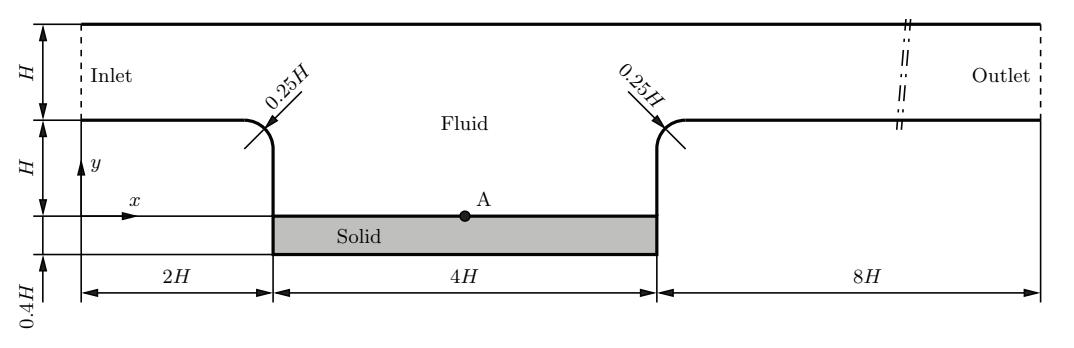
\includegraphics[scale=1]{figures/cavityFlexibleBottom-geometry}
	\caption{Channel flow over a cavity with a flexible bottom: geometry, boundary conditions and monitoring point A.}
	\label{fig:cavity_geom_m}
\end{figure}

\paragraph{Set-up.}
The flow is at $Re = 100$ and the plate is a St Venant--Kirchhoff solid, computed with the geometrically nonlinear velocity solid (\texttt{nonLinearGeometryTotalLagrangianVelocity}) on a conformal interface.
The steady state is reached by time stepping after an inlet ramp, with $\Delta t = 0.5\,\mathrm{s}$ on every level for the quasi-monolithic coupling and, as in the partitioned tutorial, $\Delta t = 0.5$, $0.25$, $0.125$ and $0.0625\,\mathrm{s}$ on levels 1--4 for Aitken coupling; the fluid uses the Euler scheme in this pseudo-time (the solid: BDF2 for the quasi-monolithic coupling and Euler for Aitken), which does not affect the steady state.
Four uniformly refined levels ($\Delta x = 0.1$, $0.05$, $0.025$ and $0.0125\,\mathrm{m}$) are computed with the quasi-monolithic coupling and with partitioned Aitken coupling under the strict convergence test.
\todo{Check the monitoring-point definition (top surface of the plate, solids4foam PR \#584) and the geometry figure against it.}

\paragraph{Measured.}
The steady vertical displacement $u_y$ of point A and the vertical interface force $F_y$ on each level for both couplings, their difference, its rate of decrease with $\Delta x$, and the Richardson-extrapolated values of each coupling; Newton iterations per step, coupling iterations per step and wall time to steady state.
A further pair of runs on levels 2 and 3 uses for the quasi-monolithic continuity flux the same face interpolation as the partitioned solver (\texttt{linear} rather than \texttt{skewCorrected linear}), which A2 identifies as the leading candidate for the remaining difference.
% A2 (a), run A1: interpolate(U) linear in system/fluid/fvSchemes.monolithic;
% also checkMesh on the final states of both couplings (run A0).

\todo{Figure: cavityFlexibleBottom. (a) Relative difference quasi-monolithic minus partitioned in $u_y$(A) and in $F_y$ (log scale) against $\Delta x$ (levels 1--4), with slope-1 and slope-2 triangles; (b) the same for the quasi-monolithic runs with \texttt{linear} continuity-flux interpolation on levels 2 and 3.}

% Data: Mx 5400191 (a421f063d), both couplings on the same build and
% monitoring point; paper-data/campaign/d/timing-ma on evidence/m-runs-d
% (timing_ma_summary.md). Time to steady: first time after which u_y(A)
% stays within 1e-4 of its final value; cost pro rata of the median
% execution time (slightly under-states Aitken, whose early steps need more
% coupling iterations). Linear-interpolation runs: evidence/m-runs-a-rfix
% (RFIX_findings.md, build 1252bd2e5, differences against the partitioned
% strict rerun).
\begin{table}[htbp]
	\centering
	\caption{Channel flow over a cavity with a flexible bottom: steady $u_y$(A) and $F_y$ with the quasi-monolithic (QM) and Aitken couplings, their relative difference $(\mathrm{QM} - \mathrm{Aitken})/|\mathrm{Aitken}|$, iterations per step and cost to steady state (one process; level 4 four processes). Last row: Richardson extrapolation with $p = 2$ from levels 3 and 4.}
	\label{tab:cavity_m}
	\small
	\setlength{\tabcolsep}{3pt}
	\begin{tabular}{lrrrrrrrrr}
		\toprule
		 & \multicolumn{3}{c}{$u_y$(A) (m)} & \multicolumn{3}{c}{$F_y$ (N)} & \multicolumn{2}{c}{Iterations/step} & Cost \\
		\cmidrule(lr){2-4}\cmidrule(lr){5-7}\cmidrule(lr){8-9}
		Level & QM & Aitken & Diff. (\%) & QM & Aitken & Diff. (\%) & QM & Aitken & QM/Aitken \\
		\midrule
		1 & $-0.203601$ & $-0.204568$ & $+0.47$ & $-5.12263$ & $-5.15280$ & $+0.59$ & 1.67 & 4.6 & 2.8 \\
		2 & $-0.231044$ & $-0.231456$ & $+0.18$ & $-5.22656$ & $-5.23915$ & $+0.24$ & 1.65 & 5.0 & 2.4 \\
		3 & $-0.238200$ & $-0.238403$ & $+0.085$ & $-5.25036$ & $-5.25660$ & $+0.12$ & 1.64 & 4.6 & 1.8 \\
		4 & $-0.239986$ & $-0.240118$ & $+0.055$ & $-5.25599$ & $-5.26008$ & $+0.078$ & 1.66 & 4.2 & 1.7 \\
		Extrap. & $-0.240581$ & $-0.240690$ & $+0.045$ & $-5.25787$ & $-5.26124$ & $+0.064$ & & & \\
		\bottomrule
	\end{tabular}
\end{table}

The steady solutions of the two couplings approach each other under refinement (Table~\ref{tab:cavity_m}): the difference in $u_y$(A) falls from $0.47\%$ on level 1 to $0.055\%$ on level 4, by a factor of 2.7, 2.1 and 1.5 per halving of $\Delta x$, and that in $F_y$ from $0.59\%$ to $0.078\%$.
Both couplings converge at second order between levels 2, 3 and 4 (ratios of successive changes of 4.0 and 4.1 in $u_y$), and their extrapolated values agree to $0.045\%$ in $u_y$ and $0.064\%$ in $F_y$, well within the uncertainty of the extrapolation itself.
The decrease of the difference slows from a factor of 2.7 to 1.5 per halving, which suggests a lower-order term among the differences of Table~\ref{tab:discretisation_differences}.
With the same continuity-flux interpolation as the partitioned solver, the difference falls from $0.18\%$ to $0.065\%$ on level 2 and from $0.085\%$ to below $0.001\%$ on level 3, which identifies the \texttt{skewCorrected} interpolation as the main cause.
\todo{Rerun the two \texttt{linear} interpolation runs on the a421f063d build and monitoring point of the table (they come from build 1252bd2e5 and the partitioned strict rerun) and add level 4, to confirm the first-order term.}
The quasi-monolithic coupling needs 1.6--1.7 Newton iterations per step on every level with the same time step, whereas the Aitken runs use the tutorial's time step, halved with each level; even so, the quasi-monolithic coupling costs 1.7 to 2.8 times as much as Aitken to reach steady state, the ratio falling with refinement as Aitken's time step falls.

%%--------------------------------------------------------------------------------------------------------------------%%
\subsection{Pulsatile compliant tube}\label{sec:womersley_consistency}
% TIME-SCHEME NOTE (Philip, 22 Oct 2026), for anyone adding results here:
% all transient results in this paper must use BDF2 (backward) for the fluid
% ddt(U) and the solid. The solids4foam tutorial default for this case is
% backward for the fluid ddt(U). Confirm and record the ddt schemes of every
% run (runs.csv); rerun any result computed with Euler, and say so here.
\todo{Time scheme: confirm that every result in this subsection uses BDF2 (backward) for the fluid and the solid (tutorial default for the fluid ddt(U): backward); results computed with Euler must be rerun.}
%%--------------------------------------------------------------------------------------------------------------------%%
% Data: the R1 womersleyTube runs (Section 4.3) and the partitioned
% Robin-Neumann and IQN-ILS runs of the companion paper, both from the tag.
% A2 (b): before the correction, the monolithic wall radial amplitude differed
% from Robin-Neumann by -3.2e-4 to -3.5e-4 (relative) on mesh factors 2 and 4
% at every step, the fluid quantities by 7e-5 or less (production CSVs
% womersleyTube_results{,_monolithic}.csv at 54a5c6916, pre-#597).

In the womersleyTube problem (Section~\ref{sec:womersley_m}) the wall deforms, so the uncorrected traction would show as a difference that does not vanish under refinement.
Both couplings are compared on mesh factors 1, 2 and 4 at 200 steps per period and on 50 to 400 steps per period on the factor-2 mesh, before and after the traction correction.

\paragraph{Measured.}
Differences between the quasi-monolithic and the Robin--Neumann and IQN-ILS solutions in every quantity of Section~\ref{sec:womersley_m}, as functions of mesh factor and time step; the difference between Robin--Neumann and IQN-ILS sets the scale of the partitioned spread.
The Fourier analysis is repeated over periods 4--5 to exclude a start-up transient.

\todo{Figure: womersleyTube, quasi-monolithic minus Robin--Neumann. Relative difference in wall radial displacement amplitude, wall phase, axial displacement amplitude and flow-rate amplitude (four markers) against mesh factor (left) and steps per period (right); open symbols before the traction correction, filled after; horizontal band for the IQN-ILS minus Robin--Neumann spread.}

Expected claims: before the correction, the wall amplitude differs by a constant \tbd{value} on every mesh and time step while the fluid quantities agree to \tbd{value}; after it, every difference \tbd{decreases under refinement / is below the partitioned spread}.
\todo{Pending reruns with the corrected traction (R1). If the correction does not remove the whole offset, report the remainder and the next candidate from A2 (partitioned coupling tolerance, run B3).}
